\documentclass[a4paper,11pt]{article}
\usepackage[slovene]{babel}
\usepackage[utf8]{inputenc}
\usepackage[T1]{fontenc}
\usepackage{lmodern}
\usepackage{amsmath, amsthm, amsfonts, amssymb}
\usepackage{graphicx}
\usepackage{float}

%%%%%%%%%%%%%%%%%%%%%%%%%%%%%%%%%%%%%%%%%%%%%%%%%%%%%%%%%%%%%%%%%%%%%%%%%%%%%

\newcommand{\set}[1]{\left\{#1\right\}} % množica
\newcommand{\abs}[1]{\left|#1\right|} % absolutna vrednost

\DeclareMathOperator{\E}{E}
\DeclareMathOperator{\PP}{P}
\DeclareMathOperator{\var}{var}
\DeclareMathOperator{\Geom}{Geom}
\DeclareMathOperator{\NegBin}{NegBin}
\DeclareMathOperator{\Student}{Student}
\DeclareMathOperator{\Fisher}{Fisher}
\DeclareMathOperator{\N}{N}
\DeclareMathOperator{\Lver}{L}
\DeclareMathOperator{\lver}{l}

\graphicspath{{./Slike/}}

%%%%%%%%%%%%%%%%%%%%%%%%%%%%%%%%%%%%%%%%%%%%%%%%%%%%%%%%%%%%%%%%%%%%%%%%%%%%%

\begin{document}

\title{Projektna naloga pri predmetu Statistika}
\author{Beno Učakar \\ Profesor: doc.~dr.~Martin Raič}
\date{}

%%%%%%%%%%%%%%%%%%%%%%%%%%%%%%%%% - Naslov - %%%%%%%%%%%%%%%%%%%%%%%%%%%%%%%%%

\maketitle

%%%%%%%%%%%%%%%%%%%%%%%%%%%%%%%%% - 1. naloga - %%%%%%%%%%%%%%%%%%%%%%%%%%%%%%%%%

\section*{1. naloga}

Nalogo rešujemo s pomočjo programa \textbf{naloga1.py}. 
Ta generira škatle z brki in za zadnji del naloge vrne:
\begin{verbatim}
    S četrtmi pojasnjena varianca dohodka družin Kibergrada
    znaša 9252923, residualna varianca pa znaša 1017132747.
    Pojasnjeni standardni odklon dohodka med četrtmi znaša 3042.
    Povprečni dohodki znašajo 45759 v severni, 41235 v vzhodni,
    37473 v južni in 42158 v zahodni četrti.
\end{verbatim}

Preučevali bomo skupni dohodek družin v mestu Kibergrad.
Imamo informacije o $43.886$ družinah, ki so v enem od štirih četrti. 
Število družin v severni, vzhodni, južni oziroma zahodni četrti je $10.149$, $10.390$, $13.457$ oziroma $9.890$.

\subsection*{Primer (a)}

Iz vsake četrti izberemo slučajni vzorec velikosti $100$. 
Na podlagi teh vzorcev narišemo škatle z brki za dohodke po četrtih, ki so prikazane na sliki~\ref{brke_po_cetrtih}.

\begin{figure}[H]
    \centering
    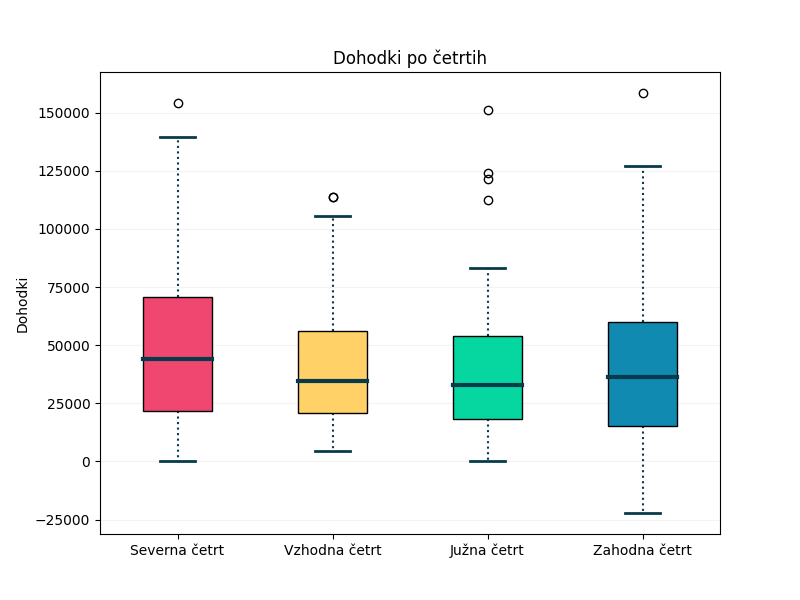
\includegraphics[scale=0.65]{Skatle_z_brki_Cetrti.png}
    \caption{Škatle z brki za dohodke po četrtih.}
    \label{brke_po_cetrtih}
\end{figure}

Najprej naredimo nekaj splošnih opazk.
Opazimo, da je variacija dohodkov znotraj severne in zahodne četrti nekoliko višja kot v vzhodni in južni četrti. 
Ker so prvi, drugi in tretji kvartil ter maksimum v severni četriti izmed vseh četrti največji, 
sklepamo, da so v povprečju dohodki v severni četrti malenkost višji od ostalih. 
V vzhodni in južni četrti je porazdelitev nekoliko nagnjena k višjim dohodkom. 
Južna četrt ima največ osamelcev, dohodki pa so izmed vseh četrti najmanj razpršeni.

Na podlagi opaženega, sklepamo, da so dohodki v severni četrti nekoliko višji kot v ostalih.
Pravtako pa se zdi, da je varianca povprečnega dohodka med četrtmi relativno majhna.
Glede na to da smo iz vsake četrti izbrali zgolj $100$ vzorcev, populacija četrti pa je v povprečju $10.000$, ti podatki niso nujno reprezentativni.
Zato s tem sklepom postopamo previdno.

\subsection*{Primer (b)}

Iz severne četrti vzamemo še 4 vzorce velikosti $100$.
Tudi za te vzorce narišemo škatle z brki prikazane na sliki~\ref{brke_sever}.

\begin{figure}[H]
    \centering
    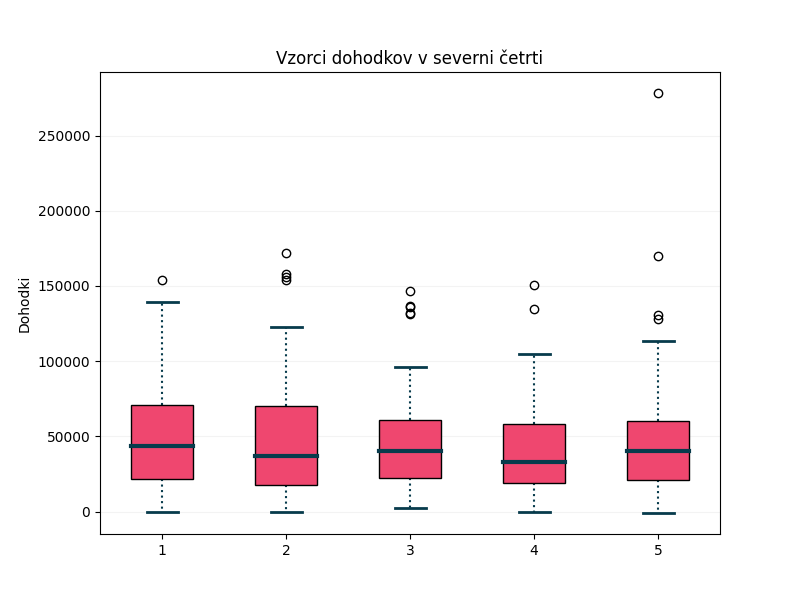
\includegraphics[scale=0.65]{Skatle_z_brki_Sever.png}
    \caption{Škatle z brki za dohodke v severni četrti.}
    \label{brke_sever}
\end{figure}

Mediane vseh škatel ležijo nad $40.000$, tako da sklepamo da večina dohodkov znaša več kot toliko.
Dohodki osamelcev znašaja v povprečju $150.000$.
Nasploh opazimo nekoliko več variacije med premožnejšimi prebivalci severne četriti.

\subsection*{Primer (c)}

Naj bo $N$ velikost populacije Kibergrada, $N_i$ velikost populacije $i$-te četrti in $w_i = \frac{N_i}{N}$ velikostni deleži četrti.
Nadaljnje naj bo $\mu_i$ povprečni dohodek in $\sigma_i^2$ varianca dohodka $i$-te četrti,
$\mu$ povprečni dohodek in $\sigma^2$ varianca dohodka celotne populacije ter $\sigma^2_p$ in $\sigma^2_n$ pojasnjena in nepojasnjena varianca celotne populacije.
Pojasnjeno in nepojasnjeno varianco pri stratificiranem vzorčenju lahko izrazimo kot
\[\sigma^2_p = \sum_{i=1}^4 w_i \mu_i^2 - \mu^2 \qquad \sigma^2_n = \sum_{i=1}^4 w_i \sigma_i^2.\]

Program \textbf{naloga1.py} vrne, da pojasnjena varianca znaša $9.252.923$, nepojasnjena varianca pa znaša $1.017.132.747$.
Pojasnjeni standardni odklon dohodka med četrtmi znaša $3.042$, kar je malo v primerjavi s povprečnimi dohodki četrti,
ki znšajo $45.759$ v severni, $41.235$ v vzhodni, $37.473$ v južni in $42.158$ v zahodni četrti.
To potrjuje hipotezo, da je razlika povprečnega dohodka družine med četrtmi majhna.

%%%%%%%%%%%%%%%%%%%%%%%%%%%%%%%%% - 2. naloga - %%%%%%%%%%%%%%%%%%%%%%%%%%%%%%%%%

\section*{2. naloga}

Nalogo rešujemo s pomočjo programa \textbf{naloga2.py}. 
Ta generira črtne grafikone in vrne naslednje podatke:
\begin{verbatim}
    Cenilka za parameter geometrijske 
    porazdelitve znaša 0.358.
    Nepristranska cenilka za parameter geometrijske 
    porazdelitve znaša 0.356.
\end{verbatim}

\subsection*{Primer (a)}

Najprej uvedimo nekaj oznak. 
Če je $k \in \set{1, \ldots, 12}$ število skokov ptic, naj bo $S_k$ frekvenca tega opažanja.
Podatke z novimi oznakami predstavimo v spodnji tabeli.
\begin{table}[H]
    \centering
    \begin{tabular}{|l|l|l|l|l|l|l|l|l|l|l|l|l|}
    \hline
    $k$ & 1 & 2 & 3 & 4 & 5 & 6 & 7 & 8 & 9 & 10 & 11 & 12 \\ \hline
    $S_k$ & 48 & 31 & 20 & 9 & 6 & 5 & 4 & 2 & 1 & 1 & 2 & 1 \\ \hline
    \end{tabular}
    \caption{Frekvence števila skokov.}
    \label{freq}
\end{table}
\noindent Skupno število opaženih skokov označimo z $S$, število vseh opažanj pa z $N$.
Velja
\[N = \sum_{k=1}^{12} S_k \qquad S = \sum_{k=1}^{12} k S_k.\]
V našem primeru znaša $N = 130$ in $S = 363$.

Želimo poiskati geometrijsko porazdelitev, ki se najbolje prilega tem podatkom. 
Naj bo število skokov pri $i$-tem opažanju slučajna spremenljivka $K_i \sim \Geom(p)$
in predpostavimo, da so spremenljivke $K_i$ med sabo neodvisne. Iščemo cenilko za parameter $p$. 
Dikcija \emph{se nejbolje prilega} nam namigne, da iščemo cenilko po metodi največjega verjetja.

Verjetnostna funkcija geometrijske porazdelitve $\Geom(p)$ je 
\[\PP(K=k) = p(1-p)^{k-1}.\]
Verjetje lahko torej izrazimo kot 
\[\Lver(p \mid K_1, \ldots, K_N) = p^N (1-p)^{S - N}.\]
Ko logaritmiramo, dobimo 
\[\lver(p \mid K_1, \ldots, K_N) = N \ln(p) + (S-N) \ln(1-p).\]
Če izraz odvajamo po $p$, enačimo z $0$ in malo računamo, pridemo do cenilke
\[\hat{p} = \frac{N}{S}.\]
Omenimo še, da bi isto cenilko dobili, če bi postopali po metodi momentov.
V našem primeru ta cenilka znaša 
\[\hat{p} = \frac{130}{363} \approx 0,358.\]
Iskana geometrijska porazdelitev je $\Geom(\hat{p})$.

\subsection*{Primer (b)}

Ob predpostavki, da so $K_i \sim \Geom(\hat{p})$, poračunamo verjetnosti $p_k$, da pri enem opažanju pride do $k$ skokov.
Pričakovano vrednosti frekvenc določimo s pomočjo programa \textbf{naloga2.py} po predpisu
\[\hat{S}_k = p_k N.\]
Dobimo spodnjo tabelo.
\begin{table}[H]
    \centering
    \begin{tabular}{|c|c|c|c|c|c|c|}
    \hline
    $k$ & 1 & 2 & 3 & 4 & 5 & 6 \\ \hline
    $p_k$ & 0,3580 & 0,2298 & 0,1476 & 0,0947 & 0,0608 & 0,0390  \\ \hline
    $\hat{S}_k$ & 46,54 & 29,87 & 19,19 & 12,31 & 7,90 & 5,07 \\ \hline
    $k$ & 7 & 8 & 9 & 10 & 11 & 12 \\ \hline
    $p_k$ & 0,0251 & 0,0161 & 0,0103 & 0,0066 & 0,0043 & 0,0027 \\ \hline
    $\hat{S}_k$ & 3,26 & 2,09 & 1,34 & 0,86 & 0,56 & 0,35 \\ \hline
\end{tabular}
\caption{Pričakovane frekvence skokov.}
\label{PricakovaneFreq}
\end{table}

\noindent Te podatke združimo v črtni grafikon prikazan na sliki~\ref{crtni_graf1}.

\begin{figure}[H]
    \centering
    \includegraphics[scale=0.7]{Črtni_grafikon.png}
    \caption{Črtni grafikon opaženih in pričakovanih frekvenc.}
    \label{crtni_graf1}
\end{figure}

Zdi se, da se pričakovane frekvence dobro prilegajo opaženim. Ponekod pride do odstopanja, 
ki pa je lahko posledica dejstva, da pričakovane frekvence $\hat{S}_k$ niso cela števila.

\subsection*{Primer (c)}

Opazimo, da je slučajna spremenljivka $S = \sum_{i=1}^N K_i$ vsota $N$ neodvisnih spremenljivk s porazdelitvijo $\Geom(p)$ 
in je zato porazdeljena negativno binomsko $\NegBin(N,p)$.
Pričakovano vrednost cenilke $\hat{p}$ lahko torej zapišemo kot
\[\E(\hat{p}) = \E\left(\frac{N}{S}\right) = \sum_{k=N}^{\infty} \frac{N}{k} \binom{k-1}{N-1}p^N(1-p)^{k-N}.\]
Ta izraz je mogoče zapisati kot vsota racionalne in logaritemske funkcije parametra $p$, vsekakor pa cenilka ni nepristranska.
Točno izražavo tu izpostimo, omenimo pa, da se zaplete predvsem zaradi faktorja $\frac{1}{k}$. 

Raje poglejmo, kaj je pričakovana vrednost slučajne spremenljivke $\frac{1}{S-1}$. 

\begin{align*}
\E\left(\frac{1}{S-1}\right) &= \sum_{k=N}^{\infty} \frac{1}{k-1} \binom{k-1}{N-1}p^N(1-p)^{k-N} \\
    &= \sum_{k=N}^{\infty} \frac{1}{N-1} \binom{k-2}{N-2}p^N(1-p)^{k-N} \\
    &= \frac{p^N}{N-1} \sum_{k=N}^{\infty} \binom{k-2}{k-N}(1-p)^{k-N} \\
    &= \frac{p^N}{N-1} \sum_{k=N}^{\infty} \binom{-N+1}{k-N}(-1)^{k-N}(1-p)^{k-N} \\
    &= \frac{p^N}{N-1} \sum_{k=0}^{\infty} \binom{-N+1}{k}(-1)^k(1-p)^k \\
    &= \frac{p^N}{N-1} p^{-N+1} = \frac{p}{N-1}
\end{align*}
Za novo cenilko parametra $p$ izberemo
\[\tilde{p} = \frac{N-1}{S-1}.\] 
Zgornji izračun pokaže, da je to res nepristranska cenilka.
V našem primeru znaša
\[\tilde{p} = \frac{129}{362} \approx 0,356.\]
S pomočjo programa \textbf{naloga2.py} ponovno izračunamo pričakovane frekvence. 
Na sliko~\ref{crtni_graf1} dorišemo še črtni grafikon novih frekvenc in tako dobimo sliko~\ref{crtni_graf2}.

\begin{figure}[H]
    \centering
    \includegraphics[scale=0.7]{Črtni_grafikon2.png}
    \caption{Črtni grafikon opaženih ter pričakovanih frekvenc s pristransko in nepristransko cenilko.}
    \label{crtni_graf2}
\end{figure}
\noindent Opazimo da se črtna grafikona prvotne in nepristranske cenilke skoraj popolnoma ujemata.



%%%%%%%%%%%%%%%%%%%%%%%%%%%%%%%%% - 3. naloga - %%%%%%%%%%%%%%%%%%%%%%%%%%%%%%%%%

\section*{3. naloga}

Nalogo rešujemo s pomočjo programa \textbf{naloga3.py}. 
Ta generira histogram in vrne naslednje podatke:
\begin{verbatim}
    Studentova statistika znaša 19.29739 in ima 
    107 prostorskih stopenj.
    Širina stolpcev po modificiranem Freedman-Diaconisovem
    pravilu znaša 20.499.
    Studentova statistika znaša 0.09837 in ima 
    (2, 43) prostorskih stopenj.
\end{verbatim}

Naj bo $P^1_i$ prvi in $P^2_i$ drugi izmerjen pulz $i$-tega študenta.
Za vsakega študenta izračunamo spremembo pulza $\Delta P_i = P^2_i - P^1_i$.
To statistiko bomo obravnavali v nadaljevanju.

\subsection*{Primer (a)}

Študente razdelimo v dve skupini glede na to ali so bili med meritvama pulzov deležni obremenitve ali ne.
Za $i = 1, \ldots, n$ spremembo pulza $i$-tega študenta, ki je bil deležen obremenitve, označimo z $X_i$. 
Podobno za $j = 1, \ldots, m$ spremembo pulza $j$-tega študenta, ki ni bil deležen obremenitve, označimo z $Y_j$.
Predpostavimo, da so razlike pulzov $X_i$ porazdeljene normalno s porazdelitvijo $\N(\mu_X, \sigma^2)$, 
razlike pulzov $Y_j$ pa normalno s porazdelitvijo $\N(\mu_Y, \sigma^2)$.

Testiramo ničelno hipotezo
\[H_0: \mu_X = \mu_Y\]
proti enostranski alternativni hipotezi
\[H_1: \mu_X > \mu_Y.\]
V ta namen opravimo T-test na testni statistiki
\[T = \frac{\bar{X}-\bar{Y}}{s_p \sqrt{\frac{1}{n}+\frac{1}{m}}},\]
kjer je 
\[s_p^2 = \frac{n\sigma^2_X + m\sigma^2_Y}{n+m-2},\]
$\sigma_X^2$ in $\sigma_Y^2$ pa sta vzorčni varianci skupin.
Program \textbf{naloga3.py} vrne, da statistika $T$ znaša $19{,}29739$ in ima $107$ prostorskih stopenj.
Iz tabel razberemo, da znašata 
\[F^{-1}_{\Student(60)}(0.05) = 1{,}671 \quad \text{in} \quad F^{-1}_{\Student(60)}(0.01) = 2{,}390.\]
Ker funkcija $F^{-1}_{\Student(k)}$ pada v odvisnosti od parametra $k$, velja
\[T > F^{-1}_{\Student(107)}(0.05) \quad \text{in} \quad T > F^{-1}_{\Student(107)}(0.01).\]

Ničelno hipotezo zavrnemo pri stopnji tveganja $0{,}05$ in $0{,}01$.
Zanesljivo lahko trdimo, da obremenitev vpliva na spremembo pulza.

\subsection*{Primer (b)}

Za spremembe pulzov študentov, ki so bili določeni za obremenitev, narišemo histogram, ki je prikazan na sliki~\ref{histogram_studenti}.
Širine stolpcov so določene v skladu z modificiranem Freedman-Diaconisovem pravilu in znašajo $20{,}499$.

\begin{figure}[H]
    \centering
    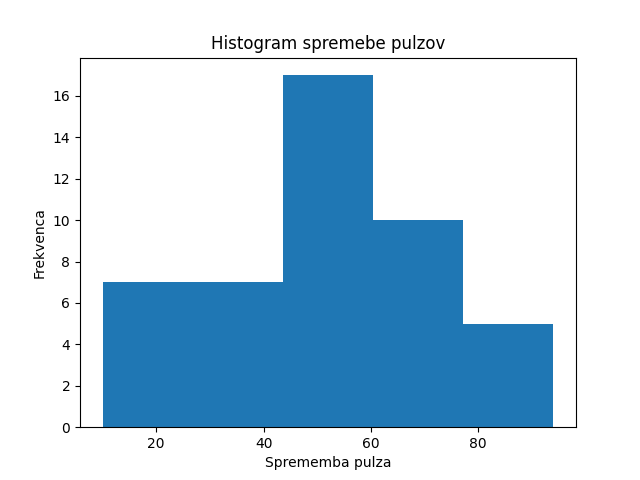
\includegraphics[scale=0.7]{Histogram.png}
    \caption{Histogram spremembe pulzov pri študentih, ki so bili določeni za obremenitev.}
    \label{histogram_studenti}
\end{figure}

Po predpostavki, naj bi bile spremembe pulzov pri študentih, ki so bili določeni za obremenitev, normalno porazdeljene.
Iz zgornjega histograma pa je razvidno, da je nekoliko več študentov imelo spremembo pulza pod $30$, kot pa bi pričakovali od normalne porazdelitve.
Zdi se, da je res nekaj študentov goljufalo.

\subsection*{Primer (c)}

Vseh $N$ študentov, ki so bili deležni obremenitve, glede na njihovo vadbo razdelimo v $k=3$ skupine. 
Z $X_{ij}$ označimo spremembo pulza $j$-tega študenta $i$-te skupine.
Predpostavimo model 
\[X_{ij} = \mu + \alpha_i + \epsilon_{ij},\]
kjer je $\mu$ pričakovana vrednost vseh meritev, $\alpha_i$ odstopanje od pričakovane vrednosti $i$-te skupine in $\epsilon_{ij}$ šum, 
za katere pa predpostavimo, da so med sabo neodvisni in porazdeljeni normalno $\N(0, \sigma^2)$.

Testiramo ničelno hipotezo
\[H_0: \alpha_1 = \alpha_2 = \alpha_3 = 0\]
proti alternativni hipotezi
\[H_1: \text{Niso vsi } \alpha_i = 0.\]
V ta namen opravimo ANOVA F-test na statistiki
\[F = \frac{\dfrac{SS_B}{k-1}}{\dfrac{SS_W}{N-k}},\]
kjer je 
\[SS_B = \sum_{i=1}^k N_i(\bar{X}_i - \bar{X})^2 \quad \text{in} \quad SS_W = \sum_{i=1}^k \sum_{j=1}^{N_i}(X_{ij}-\bar{X}_i)^2.\]
Tu smo z $N_i$ označili velikost $i$-te skupine, z $\bar{X}_i$ vzorčno povprečje $i$-te skupine in z $\bar{X}$ vzorčno povprečje vseh meritev.
Program \textbf{naloga3.py} vrne, da statistika $F$ znaša $0,09837$ in ima $(2, 43)$ prostorskih stopenj.
Iz tabel razberemo, da znašata 
\[F^{-1}_{\Fisher(2, 60)}(0.05) = 3{,}15 \quad \text{in} \quad F^{-1}_{\Fisher(2, 60)}(0.01) = 4{,}98.\]
Ker funkcija $F^{-1}_{\Fisher(2, k)}$ pada v odvisnosti od parametra $k$, velja
\[F < F^{-1}_{\Fisher(2, 43)}(0.05) \quad \text{in} \quad F < F^{-1}_{\Fisher(2, 43)}(0.01).\]
Tako ne moremo niti pri stopnji tveganja $0{,}05$ niti pri $0{,}01$ zavrniti ničelne hipoteze.
Nimamo dovolj podatkov, da bi lahko trdili, da vadba vpliva na spremembo pulza.

\end{document}
